\chapter{Configuración del vocabulario}

\textcolor{red}{ATLAS utiliza un buscador de vocabulario para realizar las definiciones de cohortes...}

El vocabualrio no viene intrinseco en ATLAS Broadsea solo viene una demo.  (see https://github.com/OHDSI/Broadsea-Atlasdb/tree/main)


\section{Descargar el vocabulario}

Para descargar el vocabulario hay que recurrir a la herramienta online de  \href{https://athena.ohdsi.org/}{ATHENA}. Este procedimiento se ha seguido gracias al forum \href{https://forums.ohdsi.org/t/downloading-omop-cdm-version-5-vocabulary-data/3321/3}{Downloading OMOP cdm version 5 vocabulary data}.

\begin{enumerate}

    \item La herramienta de ATHENA presenta un menú superior que oferta dos opciones: (a) búsqueda online en el vocabulario y (b) descarga del vocabulario. En este caso interesa descargar el vocabulario.

    \item Cuando se accede al menú de descarga \textit{Download} se presenta un listado de todos los vocabularios que contiene ATHENA entre los que algunos aparecen preseleccionados. Cada usuario puede seleccionar o deseleccionar los vocabularios que le interesen para el estudio que esté realizando. En este caso, se descargará el vocabulario que ATHENA sugiere por defecto.

    \begin{figure}[H]
        \centering
        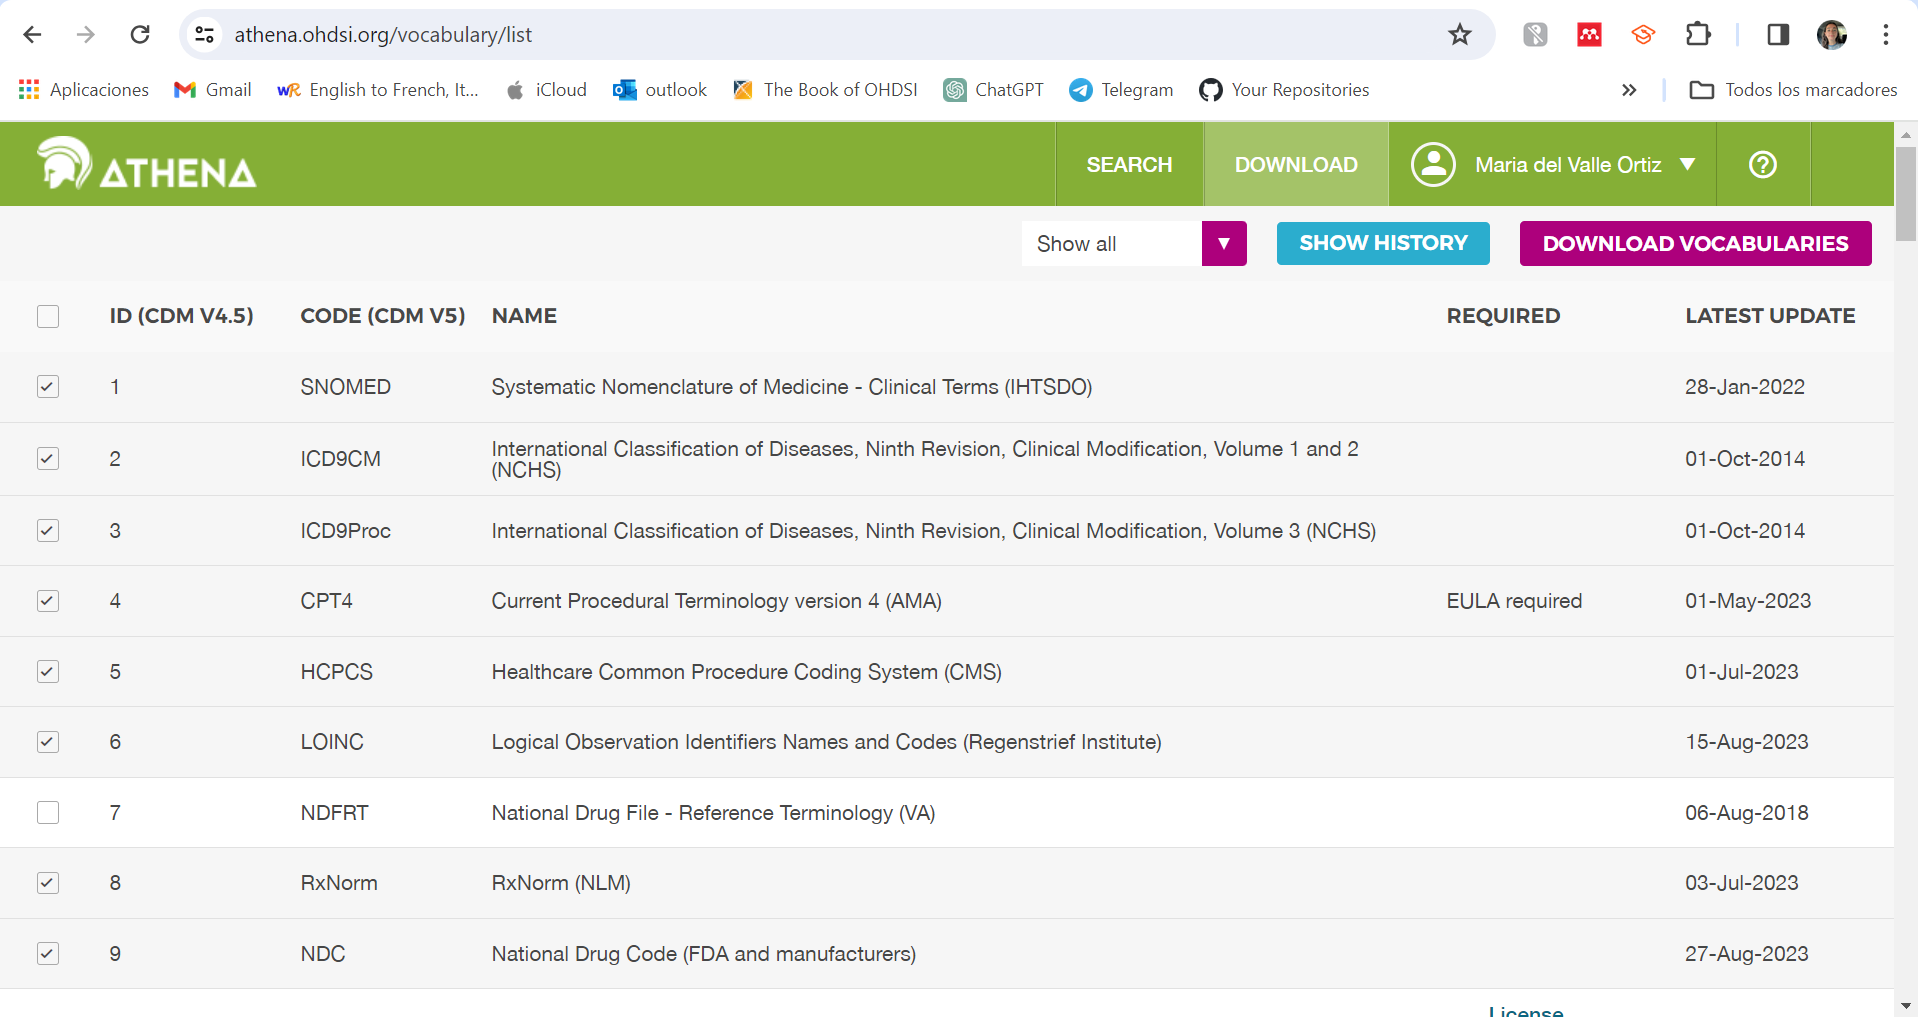
\includegraphics[width=0.90\textwidth]{figures/athenaPreDownload.png}
        \caption{Captura de pantalla de la preselección de vocabularios para descargar.}
        \label{fig:athenaPreDownload}
    \end{figure}

    \item La descarga requiere un registro de usuario con un correo electrónico válido al que se enviará un link personal que permitirá la descarga de un archivo .zip con el vocabulario seleccionado. También desde ATHENA en la pestaña \textit{''SHOW HISTORY''} muestra el estado en el que se encuentra la descarga del vocabulario y, una vez que esté listo, permite la descarga directa del zip.

    \item El archivo zip que se descarga, una vez descomprimido, muestra varios archivos .csv \textcolor{red}{con las tablas que conforman la tabla vocabulario} y \textcolor{red}{otros archivos CPT4 que no son necesarios}. Todos estos archivos deben almacenarse en el directorio local de \code{Broadsea/omop\_vocab/files}. En caso de no existir la carpeta \code{}/files, crearla manualmente. 

      \begin{figure}[H]
        \centering
        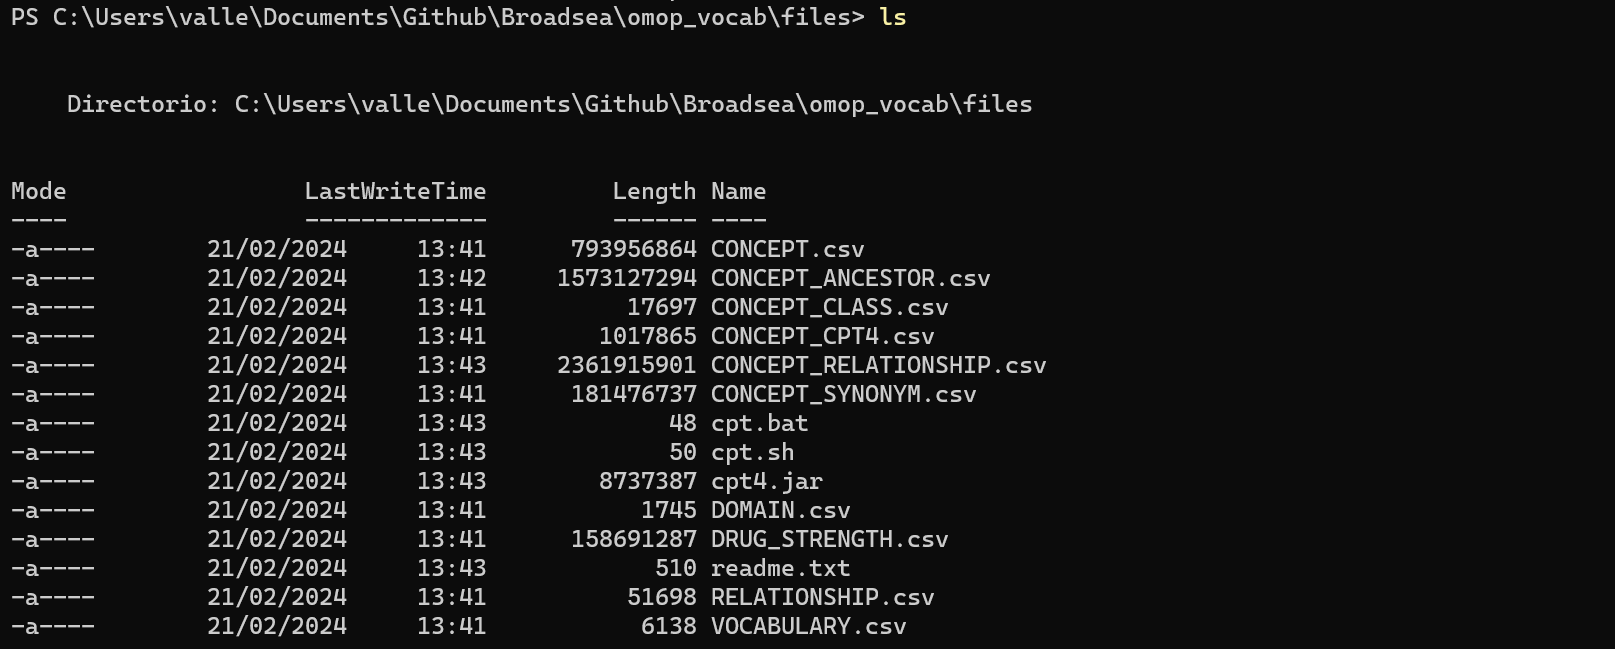
\includegraphics[width=0.90\textwidth]{figures/omopVocabFiles.png}
        \caption{Captura de pantalla de archivos descargados del vocabulario.}
        \label{fig:omopVocabFiles}
    \end{figure}

    
\end{enumerate}

\section{Configurar el vocabulario}

Configurar el vocabulario requiere acceder a la configuración avanzada del contenedor Docker. Si bien, la primera vez que se inicializó el contenedor se ejecutó el perfil \code{default} ahora se va a ejecutar específicamente el perfil \code{omop-vocab-pg-load}. Esta opción se contempla y presenta en el repositorio de Github de \href{https://github.com/OHDSI/Broadsea}{Broadsea}. 

Para acceder a la información y configuración avanzada del perfil se puede acceder al \code{docker-compose.yml} y a la sección 9 del archivo \code{.env}, aunque este caso no será necesario realizar ninguna modificación sobre los mismos.

\begin{enumerate}

    \item Para comenzar la configuración del vocabulario es necesario inicializar el contenedor \code{omop-vocab-load}. Ejecutar la siguiente línea de código en el \code{cmd}:

    \begin{lstlisting}[language=sh]
    docker compose --profile omop-vocab-pg-load up -d\end{lstlisting}

    Este comando da lugar el siguiente resultado.

      \begin{figure}[H]
        \centering
        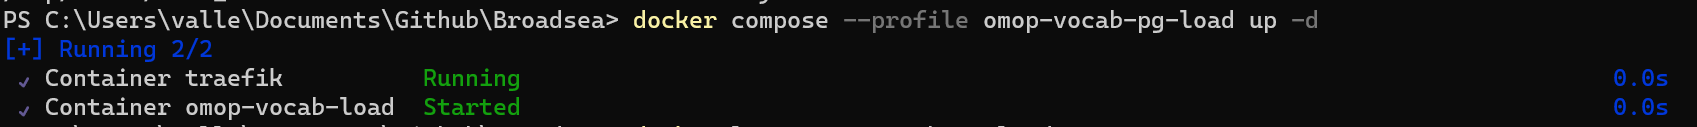
\includegraphics[width=0.90\textwidth]{figures/composeProfVocabLoad.png}
        \caption{Captura de pantalla de comando para iniciar el perfil docker.}
        \label{fig:composeProfVocabLoad}
    \end{figure}

    \item Durante la instalación del contenedor es muy importante tener abierto el \code{logs} de Docker. Se recomienda abrirlo desde Docker en vez de desde el \code{cmd} porque este último imprime el \code{logs} que se ha ejecutado hasta el momento en que se ejecuta el comando, no mantiene abierto el \code{logs} hasta que el contenedor se termine de inicializar. Sin embargo, Docker sí muestra el control en tiempo real del proceso. Proceso que ha durado 2h.

    \item La instalación 
    

    
\end{enumerate}

- Docker compose

\section{Solución de posibles errores}

- No haber creado la carpeta /files

- Haber creado la carpeta /files pero vacía

- Se crea el esquema pero se queda vacío: ESPERATE A QUE SE EJECUTE EL CONTENDOR MINIÑA